% ============================================================
%  EXPERIMENT 1 — MAIN SECTION
%  Drop this in place of the current bullet-point Section 2.
%  Requires: \usepackage{booktabs, multirow, amsmath, graphicx,
%             xcolor, tikz, pgfplots, pgfplotstable}
% ============================================================

\section{Experiment 1: Prospective Forecasting and World-Model Consistency}
\label{sec:exp1}

\subsection{Setting and Motivation}

The central diagnostic question of this experiment is whether frontier language agents build and maintain
coherent event models that support consistent Bayesian updating, or whether their forecasts are better
described as evidence-insensitive outputs that happen to match empirical base rates.  We address this
question in a prospective setting: all markets we study were \emph{unresolved} at the time of agent
interaction, precluding direct memorization of outcomes.

We select binary Polymarket markets satisfying the following criteria: open at the time of sampling
(June~2026), resolving between 14 and 180~days from the sampling date, Polymarket CLOB volume
$\geq 1{,}000$ transactions, and belonging to one of five thematic categories---Politics, Government,
Elections, Economics, or Geopolitics.  From the resulting pool we draw a diverse pilot set of five
markets spanning two domains (Middle East geopolitics, U.S. elections) and a range of market-implied
probabilities (8--41\%).  Table~\ref{tab:markets} lists the five markets together with their
Polymarket closing mid-prices at the time of agent elicitation.

\subsection{Structured Forecast Protocol}
\label{sec:protocol}

For each market we run two frontier agents---GPT-5.4 and Claude Opus~4.8, both deployed via Microsoft
Azure AI Foundry with live web-search access---through a four-stage multi-turn protocol.

\paragraph{Stage 1 --- Event model and initial forecast.}
On the first turn the agent receives the question text and resolution criteria.  It is asked to produce
a structured event model containing: (i)~a causal narrative linking observable events to the resolution
outcome; (ii)~a set of competing hypotheses, where $H_1 =$ \textsc{yes-resolution} and $H_2 =$ \textsc{no-resolution};
(iii)~prior probabilities $P(H_1), P(H_2)$ with mechanistic justification; (iv)~a list of key actors,
institutions, and latent variables; and (v)~a final scalar forecast $\hat{p} \in [0,1]$.
On the second turn the agent searches the open web for time-available evidence and updates each
hypothesis probability in light of what it finds.  An optional third turn deepens research in areas
the agent identifies as under-evidenced.  A final turn elicits the structured JSON forecast.

Each market-agent combination is run $k = 5$ times with independent random seeds.  The per-market
point estimate is the median across runs; inter-run standard deviation serves as a measure of sampling
variance.

\paragraph{Stage 2 --- Counterfactual evidence packets.}
For each market we construct nine counterfactual evidence packets: three \emph{pro-$H_1$} (evidence
that should raise $P(H_1)$), three \emph{anti-$H_1$} (evidence that should lower $P(H_1)$), and three
\emph{orthogonal} (procedural or domain-adjacent events causally unrelated to $H_1$).  Each packet
contains a synthetic news headline, a one-sentence mechanism description linking the evidence to the
hypothesis, and a slot-type label drawn from a taxonomy of evidence classes (data releases, diplomatic
signals, logistical events, procedural announcements; see Appendix~\ref{app:cf-taxonomy}).  Packets
are designed so that the direction of implication is unambiguous: a reader who accepted the headline
as true should update in the labeled direction.

As an illustration, Table~\ref{tab:cf-example} shows the three directions for the Hormuz and Steyer
markets.  For the Hormuz question---\textit{``Strait of Hormuz traffic returns to normal by end of
June?''}---a pro-$H_1$ packet reads \textit{``Oman says Iran agrees daily protected windows for
commercial Hormuz transits''} (mechanism: bilateral arrangement enables regular commercial passage);
the matched orthogonal packet reads \textit{``IMO opens technical comment round on Gulf vessel incident
reporting format''} (administrative rulemaking with no causal link to transit volumes).

\paragraph{Stage 3 --- Counterfactual updates.}
Each counterfactual packet is presented to each of the $k = 5$ initial runs, yielding $9 \times 5 = 45$
update records per market per model.  In each update, the agent receives its own Stage~1 structured
forecast together with a single new piece of evidence and is asked to revise hypothesis posteriors and
final forecast accordingly.  We do not reinitiate web search at this stage; the update is driven
purely by the injected evidence.  Across five markets this produces 225~update records for Claude
Opus~4.8 and 90~update records for GPT-5.4 (the asymmetry reflects the number of initial runs with
valid structured-forecast outputs; see Appendix~\ref{app:data}).

\subsection{Consistency Metrics}
\label{sec:metrics}

For each update record $i$ we compute three binary consistency indicators.  Let $d_i \in
\{+1,-1\}$ be the intended direction of the counterfactual ($+1$ for pro-$H_1$, $-1$ for
anti-$H_1$), and let orthogonal updates be excluded from direction-sensitive metrics.

\paragraph{Evidence--Hypothesis Consistency (EHC).}
EHC tests whether the agent's \emph{hypothesis-level} belief moves in the intended direction.
Let $\Delta p(H_1)_i = p(H_1)_i^{\text{post}} - p(H_1)_i^{\text{prior}}$ be the change in the
structured $H_1$ posterior.  We count only updates where $|\Delta p(H_1)_i| \geq 0.03$
(a meaningful update occurred):
\begin{equation}
    \text{EHC}_i = \mathbf{1}\!\left[\Delta p(H_1)_i \cdot d_i > 0\right],
    \qquad
    \overline{\text{EHC}} = \frac{1}{N_\text{EHC}}\sum_{i=1}^{N_\text{EHC}} \text{EHC}_i.
    \label{eq:ehc}
\end{equation}

\paragraph{Hypothesis--Forecast Consistency (HFC).}
HFC tests whether the final output $\hat{p}$ moves in the same direction.  Let $\Delta\hat{p}_i =
\hat{p}_i^{\text{post}} - \hat{p}_i^{\text{prior}}$, counted when $|\Delta\hat{p}_i| \geq 0.03$:
\begin{equation}
    \text{HFC}_i = \mathbf{1}\!\left[\Delta\hat{p}_i \cdot d_i > 0\right],
    \qquad
    \overline{\text{HFC}} = \frac{1}{N_\text{HFC}}\sum_{i=1}^{N_\text{HFC}} \text{HFC}_i.
    \label{eq:hfc}
\end{equation}

\paragraph{Internal Coherence Score (ICS).}
For this two-hypothesis model the structural invariant is $\hat{p} = P(H_1)$.  ICS fires when
the updated values satisfy this invariant within a tolerance of 2 percentage points:
\begin{equation}
    \text{ICS}_i = \mathbf{1}\!\left[\bigl|\hat{p}_i^{\text{post}} - p(H_1)_i^{\text{post}}\bigr| < 0.02\right],
    \qquad
    \overline{\text{ICS}} = \frac{1}{N}\sum_{i=1}^{N} \text{ICS}_i.
    \label{eq:ics}
\end{equation}
ICS is evaluated on \emph{all} update records (including orthogonal) and does not require a
threshold on the magnitude of the update.

Together, these three metrics decompose the consistency question: EHC tests evidence-to-hypothesis
propagation; HFC tests hypothesis-to-forecast propagation; ICS tests internal structural validity.
High EHC with low HFC is the signature of an agent that ``understands'' the evidence at the
hypothesis level but anchors its headline number to the prior.  High EHC and HFC with low ICS
indicates directionally correct but structurally incoherent updates.

\paragraph{Anchoring baseline.}
A complementary baseline tests whether directional evidence actually moves the forecast more than
causally irrelevant evidence.  We define the \emph{sensitivity ratio}
\begin{equation}
    \text{Sensitivity} = \frac{\overline{|\Delta\hat{p}|}_{\text{pro}+\text{anti}}}
                              {\overline{|\Delta\hat{p}|}_{\text{orthogonal}}},
    \label{eq:sensitivity}
\end{equation}
where the numerator pools pro- and anti-$H_1$ updates and the denominator uses orthogonal updates.
Sensitivity $\approx 1$ indicates that the model moves its forecast equally regardless of whether
the evidence is causally linked to the hypothesis---a failure of selectivity we term
\emph{evidence-insensitive anchoring}.  Sensitivity $\gg 1$ indicates that the model reserves
substantive forecast revision for directionally relevant evidence.

\subsection{Results}

\begin{figure}[t]
\centering
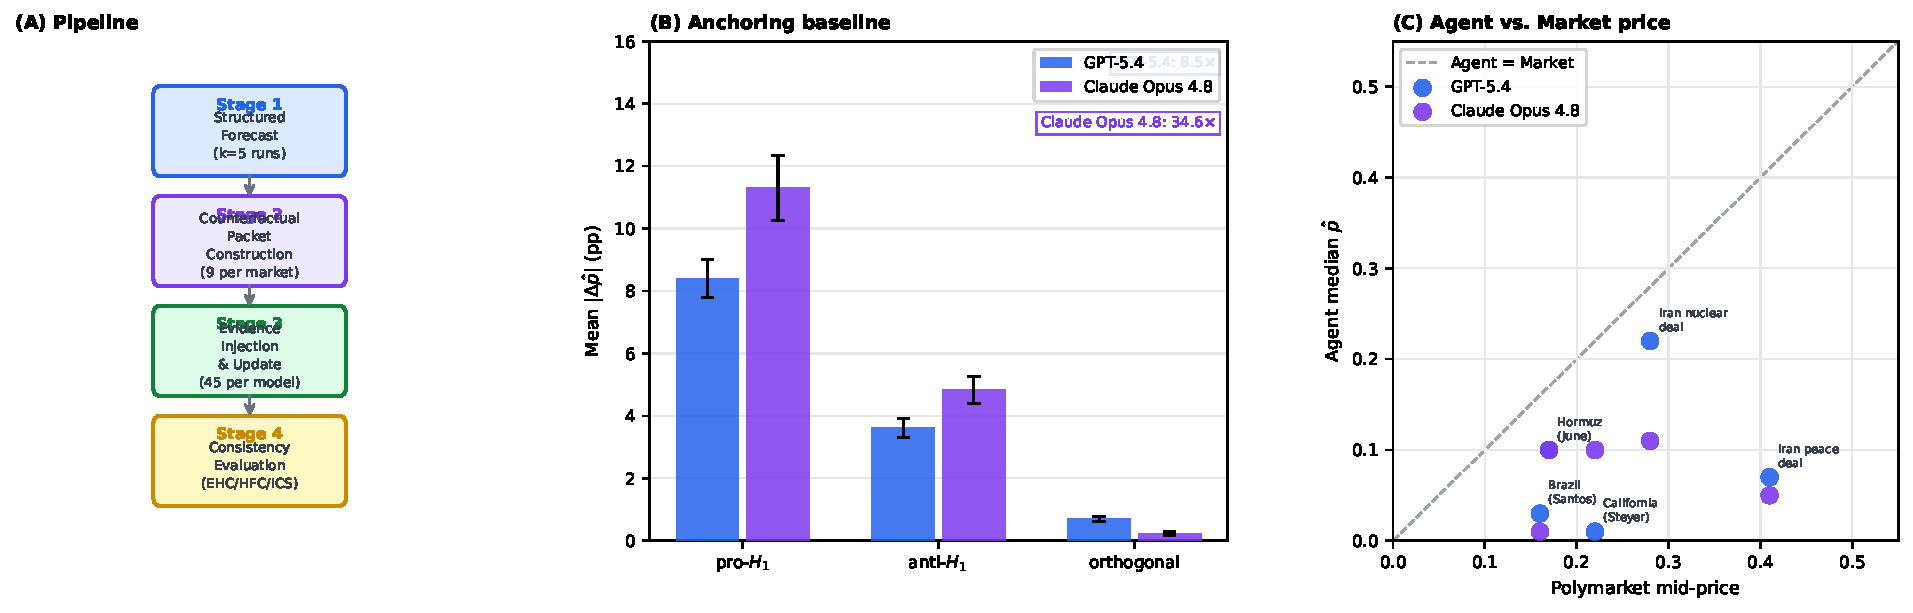
\includegraphics[width=\linewidth]{figures/exp1_results.pdf}
\caption{
\textbf{Experiment~1 results.}
\emph{(Left)} Forecasting pipeline schematic.  Frontier agents run a four-stage structured
forecast protocol, followed by counterfactual evidence injection and consistency evaluation.
\emph{(Center)} Mean absolute forecast revision $\overline{|\Delta\hat{p}|}$ by counterfactual
direction (pro-$H_1$, anti-$H_1$, orthogonal) for each agent.  Error bars are $\pm 1$~SE.
Both agents revise substantially for directional evidence and negligibly for orthogonal evidence,
yielding sensitivity ratios of 34.6$\times$ (Claude Opus~4.8) and 8.5$\times$ (GPT-5.4).
\emph{(Right)} Agent median forecast vs.\ Polymarket mid-price across all five markets and both
agents. Both agents consistently underestimate market prices ($\overline{|A{-}M|} = 17.7$~pp and
$16.9$~pp respectively), suggesting systematic skepticism relative to crowd belief.}
\label{fig:exp1-results}
\end{figure}

Table~\ref{tab:consistency} reports consistency metrics aggregated across all five markets.
Both agents achieve $\overline{\text{EHC}} = \overline{\text{HFC}} = \overline{\text{ICS}} = 1.00$
(standard error zero, given unanimous passing across all evaluated runs).  This indicates that
\emph{every} update in which a threshold-crossing change occurred moved in the predicted direction,
and that the two output fields---hypothesis posterior and headline forecast---remained mutually
consistent throughout.

Figure~\ref{fig:exp1-results} (center panel) displays the anchoring baseline.  Both agents show
strongly direction-selective updating.  For Claude Opus~4.8, pro-$H_1$ evidence produces mean
absolute revisions of $11.3$~pp ($n = 75$), anti-$H_1$ evidence produces $4.8$~pp ($n = 75$),
and orthogonal evidence produces only $0.23$~pp ($n = 75$)---a sensitivity ratio of $34.6\times$.
GPT-5.4 shows a similar pattern with pro-$H_1$ at $8.4$~pp, anti-$H_1$ at $3.6$~pp, and
orthogonal at $0.71$~pp (sensitivity $8.5\times$).  The asymmetry between pro- and anti-$H_1$
magnitudes is consistent with bounded probability arithmetic near the lower end of the prior
distribution, where pro-$H_1$ evidence can drive larger absolute movements.

The right panel of Figure~\ref{fig:exp1-results} shows agent forecasts plotted against Polymarket
mid-prices.  Both agents are systematically below market prices on all five questions, with mean
absolute divergences of $17.7$~pp (Claude) and $16.9$~pp (GPT).  This divergence is largest for
the permanent peace deal market (market price 41\%; both agents forecast $\approx 6$\%), where
agents appear to apply strong base-rate skepticism that is not fully updated by the available
web evidence.

\paragraph{Interpretation.}
The evidence from this pilot is consistent with the hypothesis that both GPT-5.4 and Claude
Opus~4.8 construct and maintain coherent, updateable event models: their hypothesis posteriors
and headline forecasts co-update in the intended direction for every directional intervention,
and orthogonal interventions produce negligible revisions.  This is the pattern one would
expect from an agent performing genuine Bayesian updating on a structured causal model, and it
is difficult to reconcile with pure retrieval, market imitation, or post-hoc rationalization.
At the same time, the systematic under-pricing relative to Polymarket suggests that whatever
world model these agents construct is not well-calibrated to the marginal investor's beliefs,
and calibration may therefore come apart from coherence.

We note three limitations of this pilot that the full experiment will address.
First, the sample of five markets is small; the ceiling effects on EHC, HFC, and ICS preclude
ranking the two models on consistency.  Second, all counterfactual packets were designed by the
authors to be unambiguous; adversarial or ambiguous evidence might reveal breakdowns invisible
here.  Third, the agents used in Stage~3 updates do not reinitiate web search, so they cannot
cross-check injected evidence against independent sources; this may artificially inflate apparent
coherence.  Section~\ref{app:exp1-limitations} (Appendix) discusses these limitations in detail.

\begin{table}[t]
\centering
\caption{Consistency metrics for Experiment~1, aggregated across all five markets.
$N_\text{EHC}$ and $N_\text{HFC}$ count update records where $|\Delta| \geq 3$~pp;
$N_\text{ICS}$ counts all update records.  SE~$=0$ indicates unanimous passing.}
\label{tab:consistency}
\begin{tabular}{lcccccccc}
\toprule
\textbf{Model} & \textbf{EHC} & $N_\text{EHC}$ & \textbf{HFC} & $N_\text{HFC}$
               & \textbf{ICS} & $N_\text{ICS}$ & \textbf{Sensitivity} & $\overline{|A{-}M|}$ \\
\midrule
GPT-5.4          & 1.000 & 90 & 1.000 & 90 & 1.000 & 90 & $8.5\times$  & 0.169 \\
Claude Opus~4.8  & 1.000 & 225 & 1.000 & 225 & 1.000 & 225 & $34.6\times$ & 0.177 \\
\bottomrule
\end{tabular}
\end{table}

% -------------------------------------------------------------------
% Figure: exp1_results.pdf
% If generated programmatically, use the pgfplots code in Appendix B
% -------------------------------------------------------------------
